\documentclass[]{article}
\usepackage{../macros}

\usepackage{biblatex}
\addbibresource{sources.bib}

\head{Project Defense}
\begin{document}

\setlength{\parskip}{12pt}

% -- Title Page --
\begin{titlepage}
  \begin{center}
  \textbf{\Huge Kazooformation} \par
  \vspace{0.5cm}
  \textit{An engaging teaching tool for the lowest layer of the OSI model} \par
  \vspace{1.5cm}
  \textbf{Joshua Jerred} \par

  % QR Code
  \vspace{4cm}
  
\includegraphics[width=0.2\linewidth]{images/qr.png} \par
  \textit{https://kazooformation.joshuajer.red}

  \vfill % Fill the remaining vspace

  \text{Utah Tech University} \par
  \text{CS-4600 Senior Project} \par
  \textbf{24 April 2025}

  \end{center}
\end{titlepage}

% ------------------------------------------------------------------------------
\section{The Problem}

% The problem that was addressed by this project. Give enough information for the importance of the problem to be clear. Do not include “I was going to” information.


Computer Science students are familiar with the OSI model, but often the details of the lowest layer, the physical layer, are glossed over. This is normally left to the electrical or computer engineering students. In the modern world we are seeing a shift towards software defined networking, where the physical layer can be controlled by flexible software instead of rigid hardware\cite{ibmWhatSoftwareDefined}. An example of this is the Joint Tactical Radio System (JTRS), which is a software defined radio program that was started by the US Department of Defense in the 1990s and is still being developed today\cite{Cox_2001}. It's clear that there is a need for a better understanding of the physical layer as software solutions are becoming more common.


Unfortunately, the broad fields of Digital Signal Processing (DSP) and Information Theory are riddled with trigonometry and dense with acronyms that can be difficult to learn. This results in a challenging path towards developing the base intuition that is required to learn advanced DSP topics.

Generally, the more engaging a teaching tool is, the more value it can provide as it's easier for early learners to connect with the topic. Therefore, an engaging physical layer teaching tool can be created based on the following assumptions:

\begin{itemize}
  \item[1.] DSP and information theory are often perceived as difficult and unengaging topics.
  \item[2.] Kazoos are not boring.
\end{itemize}

% ------------------------------------------------------------------------------
\section{The Solution}

% The features and functionality that were implemented and working. This must include a video segment that demonstrates the working software, with a voice description. Include all elements you wish to be graded on.

% The text document must include a link to the source code repository(s). If applicable, a link to the live application and instructions for use must be included.

The choice to utilize the kazoo is a simple one - it makes the topic a lot more fun. This was inspired by the paper "Harder Drive: Hard drives we didn't want or need", by Dr. Tom Murphy VII, which enabled learning about topics that many otherwise wouldn't have learned about if it wasn't for a "needless"\cite{murphy2022harder} approach.

The goal of this project was to create a new physical layer that can be heard and felt by the user, for the purpose of explaining fundamental DSP and signal processing topics. This was done by creating a software system that uses kazoo sounds to encode, store, and decode data as a series of discrete kazoo signals. This system is called Kazooformation.

Kazooformation uses recorded kazoo sounds to encode and decode data. Different
sounds are used to represent different bits, and the series of sounds can be
used to represent a byte stream. This is all audible, so the user can hear the
data being transmitted, making it possible to see the physical layer in action.

\begin{center}
  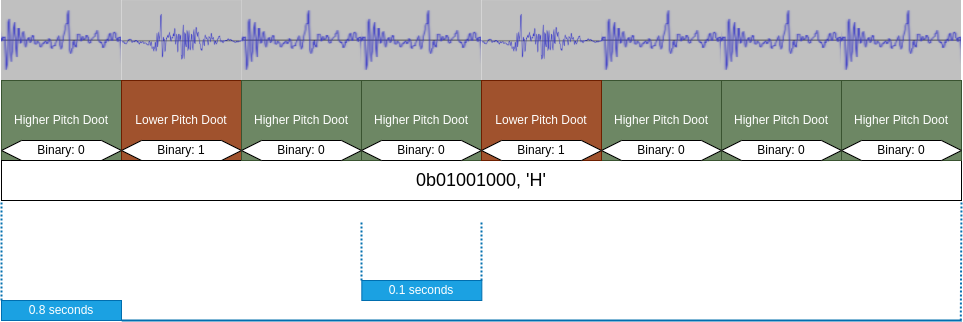
\includegraphics[width=0.7\linewidth]{images/kazoo_signal.png}

  \textit{Figure 1: The ASCII letter "H" encoded as a kazoo signal using a binary model.}
\end{center}

Ultimately, Kazooformation is based on Audio Frequency Shift Keying modulation, which means that the concepts directly map to real world modulation applications.

\subsection{Kazoo Translation Layer (KTL)}

\begin{center}
  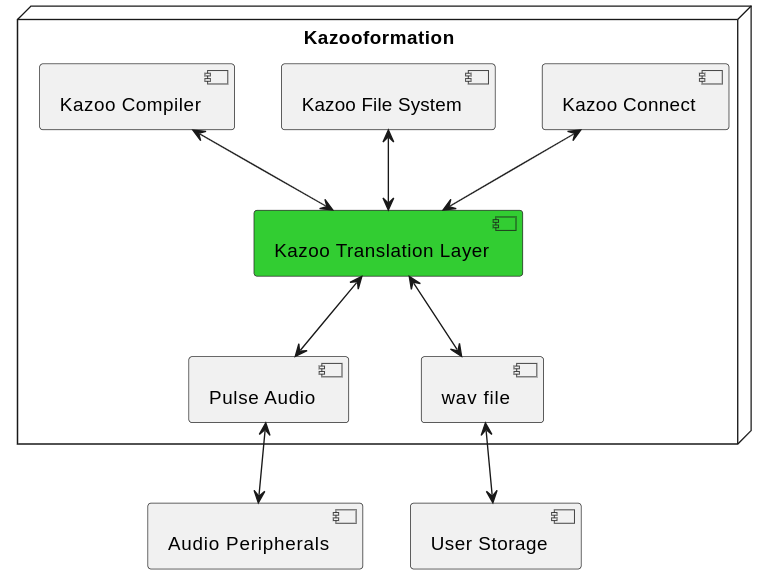
\includegraphics[width=0.4\textwidth]{images/org_diagram.png}

  \textit{Figure 2: The Kazooformation system architecture.}
\end{center}

KTL is a software library that is the core of the Kazooformation system. It is responsible for converting between serialized data and kazoo signals. As an abstract layer, it can be applied to a wide range of applications; if you have a byte stream, it can be converted to kazoo signals and back.

The most important detail of the KTL is the model system which is leveraged to use different symbols to represent different bits depending on the application. This enables flexibility in choosing symbol sets, symbol rates (baud), and bit rates, depending on channel limitations (e.g., audio cable vs. open air playback).

Although the focus was on the physical layer, the KTL offers a simple frame/packet structure that can be used as a simple data link layer.

\subsection{Kazoo Connect (Chat Client)}

Kazoo Connect is a simple terminal and/or web based chat client that uses the KTL to send and receive text messages using kazoo sounds. Its purpose is to demonstrate the KTL in a real world application. It uses the user's default audio input and output devices as the communication channel.

There is also a basic HTTP server that keeps track of received messages, allowing for a simple web interface to be used. The web client is a minimal React-based web client that provides a friendly interface for non-technical users.

\subsection{The Code and How to Build It}
Kazooformation repo: \url{https://github.com/joshua-jerred/kazooformation}

All build and use instructions can be found in the file README.md, located in the root of the repository. Kazoo Connect works on Linux and MacOS.


% ------------------------------------------------------------------------------
\section{Technical Overview}

% The strategy employed by your solution to this problem. Give enough information that someone reading the source code will have context to understand what algorithms and architecture are being implemented. Do not include “I was going to” information.

% Provide information on environments, languages, and algorithms used for this project.

This project is dependent on the Kazoo Translation Layer, all applications are built on top of it. It builds and works on both Linux and MacOS, but the development was done on Linux. The CMakeLists.txt file in the root of the repository is the best place to look to understand file structure.

\miniheader{Term Definitions}
\begin{itemize}
  \item \textbf{Symbol}: A symbol is a discrete kazoo sound that can be used to represent a bit or a series of bits.
  \item \textbf{Model}: A model contains a unique set of symbols, their corresponding bit values, and the modulation scheme used to encode the symbols.
  \item \textbf{Baud Rate or Symbol Rate}: The rate at which symbols are transmitted and received. Baud and symbol rate are used interchangeably. This is \textit{not} the same as bit rate as multiple bits can be represented by a single symbol.
  \item \textbf{Bit Rate}: The rate at which bits are transmitted and received. This is defined as $\text{Baud Rate} \times \text{Number of Bits per Symbol}$.
  \item \textbf{Symbol Level Alignment}: The process of detecting the start and end of a symbol in a stream of audio data. Required for decoding the symbols from unaligned audio data. WAV files are assumed to have symbol-aligned data, so alignment issues are minimal in that context.
  \item \textbf{FFT}: Fast Fourier Transform, an algorithm that converts a signal from the time domain to the frequency domain. See the image below.
  \item \textbf{Frequency Peak}: If an FFT is taken across audio samples, the peak frequencies can be detected. These are the audio frequencies that are most present in the audio samples.
\end{itemize}

\begin{center}
  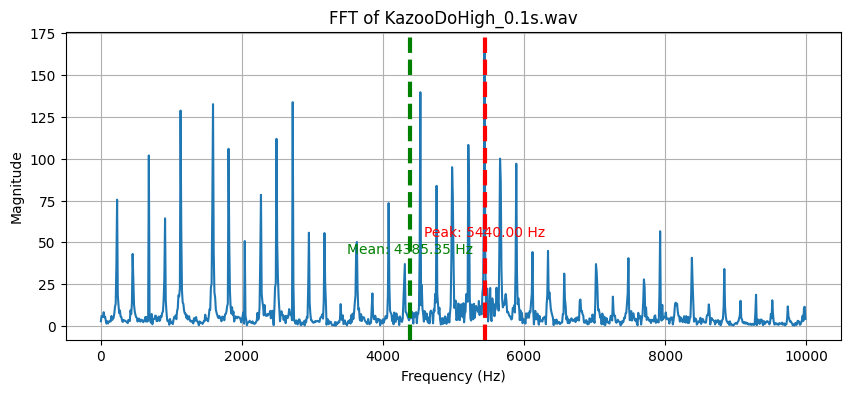
\includegraphics[width=0.7\linewidth]{images/fft.png}

  \textit{Figure 3: An FFT of a kazoo sound, with the peak frequency marked by a red line.}
\end{center}

\subsection{The Kazoo Translation Layer}

The KTL was created as a C++ library using the CMake build system. Being a CMake interface library, it can easily be used in other CMake projects. A user of this library only needs to include the header ktl/translation\_layer.hpp

\miniheader{Software Stack}
\begin{itemize}
  \item \textbf{Toolchain}: C++17, CMake, GNU/GCC.
  \item \textbf{FFTW-3}: A C library for Fast Fourier Transforms/audio signal analysis.
  \item \textbf{PulseAudio}: A C library for audio input/output.
  \item \textbf{GTest/GMock}: A C++ library for unit testing.
\end{itemize}

\miniheader{Key Software Components}
\begin{center}
  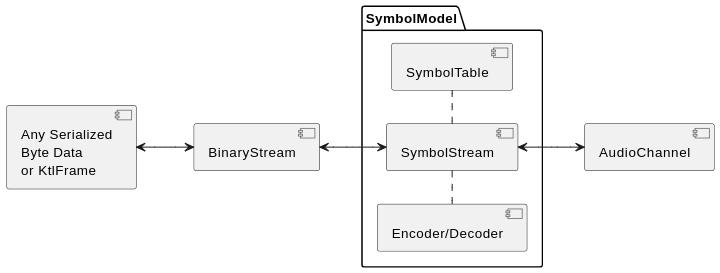
\includegraphics[width=0.8\linewidth]{images/ktl_flow.png}

  \textit{Figure 4: The data flow of the Kazoo Translation Layer.}
\end{center}

\begin{itemize}
  \item \textbf{AudioChannel}: A generic interface for continuous 16-bit PCM audio samples. This is used to allow for easy integration of different audio input/output software. It is used for both WAV files and PulseAudio. The audio channel interface is used by the model to encode and decode audio samples to/from the \textbf{SymbolStream}.

  \item \textbf{SymbolStream}: The symbol stream is a simple double ended queue that is used to store the symbols that are being transmitted and received. The symbol stream can be converted to and from a \textbf{BinaryStream}. Each model has a unique symbol stream (templated) as the symbols and their bit-width are defined by the model.

  \item \textbf{BinaryStream}: The binary stream is a class that is used to store raw binary data where the concept of a byte is abstracted away. This is important to keep the model system bit-width agnostic. It allows for easy serialization and deserialization of data.

  \item \textbf{SymbolModel}: This is the base class for all kazoo models. It contains the symbol set and stream, a mapping of symbols to bits, and the modulation scheme used to encode/decode the symbols. To implement a new model, a copy of an existing model can be made and added to the model list.

  \item \textbf{KtlFrame/Deframer}: KTL isn't supposed to go past the physical layer, but a simple frame structure is provided to allow for easy integration. The frame has unique start and end bytes (outside of 7-bit ASCII) to allow for easy detection of the start and end of a frame. The frame is converted to and from a \textbf{BinaryStream}. The frame structure is accessible to the users of the KTL.

\end{itemize}

\miniheader{Test Driven Development}

As KTL is primarily an abstract library, test driven development is necessary. The majority of the KTL is unit tested using GTest and GMock.

\miniheader{The Models \& Modulation Schemes}

A few models have been created inside of the KTL. They can be found in the \texttt{src/ktl/models} directory. All models use the FFT wrapper created in the file \texttt{src/ktl/audio/fft.hpp} for signal analysis.

When it comes to encoding, the kazoo models take the provided BinaryStream and convert it to a symbol stream. The symbol stream is then processed in order; each symbol is mapped to PCM audio samples that are used to populate the generic audio channel.

All models operate at a fixed symbol rate of 10 symbols per second; this rate ensures the resulting signal remains audibly distinguishable and pedagogically effective. This is a somewhat arbitrary choice, individual models can use different symbol rates at the cost of reliability.

\begin{itemize}
  \item \textbf{TestingModel}: A non-kazoo binary model (two symbols, representing 0 and 1) that is used for unit testing. It does not provide symbol level alignment. It encodes data as simple sine waves.

  \item \textbf{K1 Model}: The first kazoo model to use actual kazoo sounds. It is a binary model without symbol level alignment. It simply checks if the peak frequency of the signal is above or below a center frequency. This model is best suited for pre-recorded kazoo signal .wav files.

  \item \textbf{K2 Peak Model}: A 4-symbol kazoo model that uses a basic frequency peak detection algorithm to differentiate between the symbols. This model provides basic symbol level alignment. This is the most efficient model when using WAV files. Although it has symbol alignment, it is not very reliable due to the nature of kazoo sounds and the audio samples chosen for the symbols. This means that PulseAudio works, but the underlying audio channel must be near perfect (e.g. no open air communication).

  \item \textbf{K3 Reasonable Model}: A binary kazoo model that focuses on functionality over performance, allowing for open air communication between devices. Although the software is similar to the K2 model, the symbol audio samples were carefully recorded and chosen to be more distinct and consistent. This model has better symbol level alignment than the K2 model; across the length of a single symbol, multiple FFTs are taken to determine where one symbol ends and the next begins. This model has the most robust test coverage as well.

  The same peak detection algorithm is used in this model as even with carefully chosen audio samples, different peak frequencies can be detected in the same symbol. There is a good opportunity for improvement here.
\end{itemize}

\subsection{Kazoo Connect}

Kazoo Connect is just an application example of the KTL, it was intentionally kept simple. The terminal and web client/server are separate applications but they can communicate with each other.

\miniheader{Kazoo Connect Terminal}

Kazoo Connect Terminal is a simple terminal client with a thread for KTL and a thread for the user input. All code for this is in the file \texttt{src/main.cpp}. It can be built and run using the target \texttt{kazoo\_connect}.

\miniheader{Kazoo Connect Server}

Kazoo Connect Web is similar to the terminal client but it provides a simple HTTP server for use with a web client. The server uses basic TCP socket handling with minimal parsing of the HTTP protocol. The server has paths for getting all received messages and status, sending a message, and clearing the list of received messages. The server can be built and run using the target \texttt{kazoo\_connect\_server}.

The web client is a simple React app that is derived from the create-react-app template with a basic form to send messages and a list of received messages. It can be run like any other node js application from the \texttt{src/kazoo\_connect\_server/web\_client} directory. API requests are proxied to the backend.


\subsection{Using KTL in Other Projects}

Thanks to CMake, KTL can easily be used in other projects. Here are two simple examples that demonstrate KTL integration into other applications:

\miniheader{Example: Creating a CMake target that uses the KTL}
\begin{verbatim}
  # An application that uses the Kazoo Translation Layer
  add_executable(kazoo_connect src/main.cpp)
  target_link_libraries(kazoo_connect kazoo_translation_layer)
\end{verbatim}


\miniheader{Example: Writing data to a .wav kazoo file}
\begin{verbatim}
  // Any type that can be converted to a std::span can be used
  const std::array<uint8_t, 4> data = {0, 1, 2, 3};

  kazoo::TranslationLayer tl{kazoo::TranslationLayer::ModelType::K3_REASONABLE_MODEL};
  tl.addData(data);
  tl.encode();
  tl.saveWav("test.wav");
\end{verbatim}

\subsection{Audio Analysis Work}

There was a large amount of work done to analyze the audio samples that were recorded and used in the KTL. This can be found in the \texttt{doc/} directory.Most of the work was done using Python along with various audio processing libraries.

Kazoo sounds are awfully noisy and inconsistent, FFT visualizations were critical for selecting the best audio samples and for knowing where their frequency peaks were.


% ------------------------------------------------------------------------------
\section{Research Summary}
% A list of resources and references used in completing the project. For example, articles, books, interviews/meetings, tutorials, videos, etc. For each one, include a description and a reason for using it (what knowledge/skill did you gain from the resource?).

\begin{itemize}
  \item \textbf{https://kazoologist.org} - This website is one of the only resources available for kazoo research. It was incredibly helpful for understanding what was actually going on at the sound level.

  \item \textbf{Meetings with Curtis Larsen} - Regular meetings with Curtis were critical for keeping the project on track and resolving project planning issues.

  \item \textbf{Meeting with Bart Stander} - After mentioning my project to Bart, he provided me with the mathematical background for understanding music notes within an octave. This was helpful for getting unstuck in the early signal analysis phase and it helped with planning signal differentiation.

  \item \textbf{Wikipedia (Modulation Pages)} - Wikipedia is seemingly the best place to read about information theory and DSP concepts. The signal modulation page maps out a large number of high level concepts. It helped me connect the necessary dots between the various concepts.

  \item \textbf{StackOverflow} - StackOverflow was most used for figuring out how to use the FFTW-3 library. It of course was a constant companion and deserves a mention.

  \item \textbf{NoiseCollector on freesound.org} - The user NoiseCollector on freesound.org has a few kazoo audio files that were used to create the initial models before custom samples were recorded.

  \item \textbf{https://notblackmagic.com} - This website provides written tutorials on various DSP concepts including filtering and modulation/demodulation.

  \item \textbf{My Past Work} - In the past I have used Pulse Audio, WAV files, and TCP sockets. I pulled the initial code for these components from my past work.
  
  \item \textbf{Dr. Tom Murphy VII} - Without the paper "Harder Drive: Hard drives we didn't want or need", I would have never considered a 'needless' approach to developing learning tools.

  \item \texttt{https://www.youtube.com/watch?v=h7apO7q16V0} - This video was a great refresher on FFTs and how they work, needed for FFTW-3 usage.

  \item \textbf{Monoprice} - Like all other networking equipment, Monoprice sells kazoos, they're decent quality and cheaper than Amazon.

\end{itemize}

% ------------------------------------------------------------------------------
\section{Further Work}

% Briefly list the next steps you or someone else might take to extend this work.

Kazooformation is a functional system, but there is certainly a lot of room for improvement within the KTL.

\begin{itemize}
  \item The various models can be parameterized to allow for different symbol rates and bit rates. There is clearly an opportunity for a machine learning model here. For example, a model could be trained to maximize symbol separation in the frequency domain under various noise conditions.

  \item The demodulation algorithm should be improved. The current algorithm relies on a naive approach to peak detection and it is not very reliable. An approach that properly applies various filters to the signal should be used.

  \item An 8-symbol or 16-symbol model could be designed with new audio samples to improve bit rate.
\end{itemize}


% Although I have some experience with C++ and some with DSP, using kazoo signals creates
% a unique challenge which will test my abilities. The C++ FFT library in entirely
% new to me. I think the kazoo adds a unique challenge performance and reliability wise. This project will require for me to learn more about performant implementation while doing DSP. \\

% Unit testing will prove to be very helpful for this project, I plan on using GTest and GMock as needed.

% On the kazoo side of things, the website http://kazoologist.org/ has done the vast majority of the leg work when it comes to kazoo research. This is legitimately a helpful resource as it provides crucial information related to creating unique sounds. I sent an email to this person about a month ago and sadly did not receive a response.


%  ------

% After some initial research, it's been shown that kazoos are one of the worst carriers for creating distinct audio signals. Below are output graphs from a Fast Fourier Transform (FFT) across two audibly distinct kazoo samples. It can be seen that the audio is very messy and some effort will need to be put into finding a reliable way to differentiate between distinct kazoo signals.

% \CenterImage{fft_1.png}[0.5\textwidth]

% \CenterImage{fft_2.png}[0.5\textwidth]

% Another mathematical reality is the fact that at least 0.005 seconds of audio data is required to get the full scope of each kazoo sound, which can be seen in the waveform below (repeating patterns that are ~0.005s long).

% \CenterImage{waveform_1.png}[0.8\textwidth]

% Due to this, the fundamental symbol rate limit of a kazoo based communication
% system is 200 symbols per second. With this symbol rate limitation, if there
% were only two distinct symbols, representing $1$ and $0$, the bit rate would be
% 200 bps which is nearly unusable. Thankfully, kazoos are capable of generating
% all sorts of different noises, so we can create as many distinct symbols as we
% want, allowing us to encode multiple bits at once. We are only limited by the ability to differentiate between distinct symbols. The more symbols we have, the higher the data rate, but the error rate will increase as well. \\

% \begin{itemize}
%   \item[Weeks 1-2]: Create the basic project structure, build basic targets with all libraries linked (FFTW-3 \& GTest/GMock). Also, buy a kazoo and start creating symbols.
%   \item[Weeks 3-4]: Start work on the Kazoo Transition Layer, basic unit tests. This will be the majority of the FFT work and will be the greatest challenge. Two unique symbols should be the initial goal.
%   \item[Week 5-6]: Create a basic symbol identifier that can differentiate between at least 4 kazoo signal symbols.
%   \item[Weeks 6-9]: Kazoo Translation Layer reliability and bit rate maximization - unit testing with introduced noise for later use over unreliable channels.
%   \item[Weeks 10-11]: Kazoo Connect - unit test and manual testing using two separate computers in the same room.
%   \item[Weeks 11-12]: Kazoo File System - Create the basic wav file wrapper, consider a nested structure.
%   \item[Weeks 12-15]: Kazoo Translation Layer automatic channel quality monitoring and dynamic strategy management. Make the symbol rate/number of symbols non-static, so if the quality of the underlying communication channel worsens, the data rate will be slowed down to compensate for a high bit error rate and vice versa. There is a large chunk of time reserved for this as this period is focused on pushing the KTL to it's limits. Consider an RTP (Reliable Transport Protocol) approach depending on the time that is available.
%   \item[Stretch Goal]: Kazooxecutable: Integrate the kazoo translation layer into the compiler from CS-4550.
% \end{itemize}

% \section{Validation Plan}

% Continual validation should be done via Unit Testing. The Kazoo Translation Layer should be fully unit tested as it is the basis of the whole system. This is a highly testable system, so there should be no problems achieving a target of 90\% test coverage within the translation layer. The applications built on top of the translation layer can also be unit tested, but it may not be as valuable as they can be tested manually.

% The other components should go through manual testing - it will be clear if they work or not.

% \begin{itemize}
%   \item File System - Can a file be wrapped on one client, sent to another, and be unwrapped?
%   \item Chat Client - Can two people have a typing-speed text conversation via a Discord call using the Kazoo chat client?
%   \item Compiler - Can applications be built and then later run from wav files?
% \end{itemize}



\printbibliography

\end{document}